\documentclass{article}
\usepackage{amsfonts}
\usepackage{amssymb}
\usepackage{url}
\usepackage{hyperref}
\usepackage{amsmath}
\usepackage{centernot}
\usepackage[utf8]{inputenc}
\usepackage[russian]{babel}

\title{Сложности вычислений. Полиномиальный алгоритм раскраски 3-раскрашиваемого графа в $O(\sqrt{n})$ цветов}
\author{Ульянин Дмитрий, 597}
\date{Декабрь 2017}

\usepackage[square,numbers]{natbib}
\usepackage{graphicx}
\usepackage{listings}

\newtheorem{theorem}{Теорема}
\newtheorem{lemma}{Утв.}
\newtheorem{definition}{Определение}

\begin{document}

\maketitle

\section{Вступление}
\begin{definition}
	
	Смежные вершины (соседи) вершины $v$ графа $G$ будем обозначать $N(v)$.
	
	Степернь вершины обозначим $deg(v)$.
	
	Степень максимальной вершины графа $\Delta(G)$.
	
	Раскраской графа $G = <V, E>$ назовем функцию ${color : V \rightarrow int}$.
	
    Раскраска графа называется *правильной*, если ни одно ребро не соединяет вершины одного цвета.
\end{definition}

Известно, что задача поиска правильной раскраски графа в $k$ цветов при ${k > 2}$ является $NP-$полной.

\begin{theorem}{Кёнига, б/д}
	
	Граф $G$ является двудольным тогда и только тогда, когда все циклы в графе G имеют чётную длину.
\end{theorem}

\begin{lemma}
    Проверка графа на двудольность и нахождение раскраски в 2 цвета лежат в $\mathbf{P}$.
\end{lemma}
\paragraph{Доказательство}
	Граф $G$ можно раскрасить ровно в 2 цвета $\iff$ $G$ двудольный $\iff$ $G$ все циклы четной длины $\iff$ алгоритм обхода графа <<не ходит>> в серую вершину, до которой расстояние нечетно.
	
	Таким образом, чтобы найти 2-раскраску, можно запустить $dfs(v)$, во время которого красить соседей $v$ в цвет, противоположный $color(v)$ (в $\mathbb{Z}_2$). Если же в какой-то момент вершина красится в цвет соседа, то граф не двудолен.
	
	Алгоритм покраски в два цвета назовем $\textbf{B}$.

\section{Жадный алгоритм, \textbf{G}}
\begin{definition}
    *Жадным* назовем следующий алгоритм:
    \begin{enumerate}
    	\item for i = 1 .. n:
    	\item C = $\cup_{j<i\ :\ j \in N(i)} {color(j)}$ -- множество цветов соседей $i$ с меньшим номером
    	\item $color[v] = mex(C)$ где $mex(C)$~--- это первый цвет, которого нет в C.
    \end{enumerate}
\end{definition} 

\paragraph{Доказательство корректности}
Следует из того, что выбираем цвет, которого нет среди соседей
\hfill

\begin{lemma}
    Пусть максимальная степень вершины в графе $d$. Тогда жадный алгоритм раскрасит граф в не более чем $d + 1$ цвет.
\end{lemma}
\paragraph{Доказательство}
$\forall v \in V$ $color(v) \leq deg(v) + 1$ так как вершину соседей вершин $v$ не больше $deg(v)$, а значит всегда найлдется отличный от них цвет, кототорый будет $deg(v) + 1$-ым.

\section{Алгоритм Вигдерсона, \textbf{W}}

\begin{theorem}
    Раскраска 3-раскрашиваемого графа в $O(\sqrt{n})$ цветов возможна за полиномиальное время.
\end{theorem}

\begin{definition}
    Рассмотрим следующий алгоритм:
   
    \begin{enumerate}
    	\item Пусть $c$ = 1
    	\item $\Delta(G) \geq \sqrt{n}$: Рассмотрим $v$ т.ч. $deg(v) \geq \sqrt{n}$. Если такой нет, перейдем к шагу 3. 
    	
    	Используем алгоритм $\textbf{B}$, чтобы раскрасить $N(v)$ в $k \in \left\{1, 2\right\}$ цветов: $c$ и $c + 1$. Удалим из графа $G$ вершины $N(v)$. Обновим $c += k$.
    	
    	\item $\Delta(G) \le \sqrt{n}$: Используем алгоритм $\textbf{G}$ жадной раскраски, чтобы раскрасить оставшиеся вершины.
    \end{enumerate}
   
\end{definition}
\begin{center}
	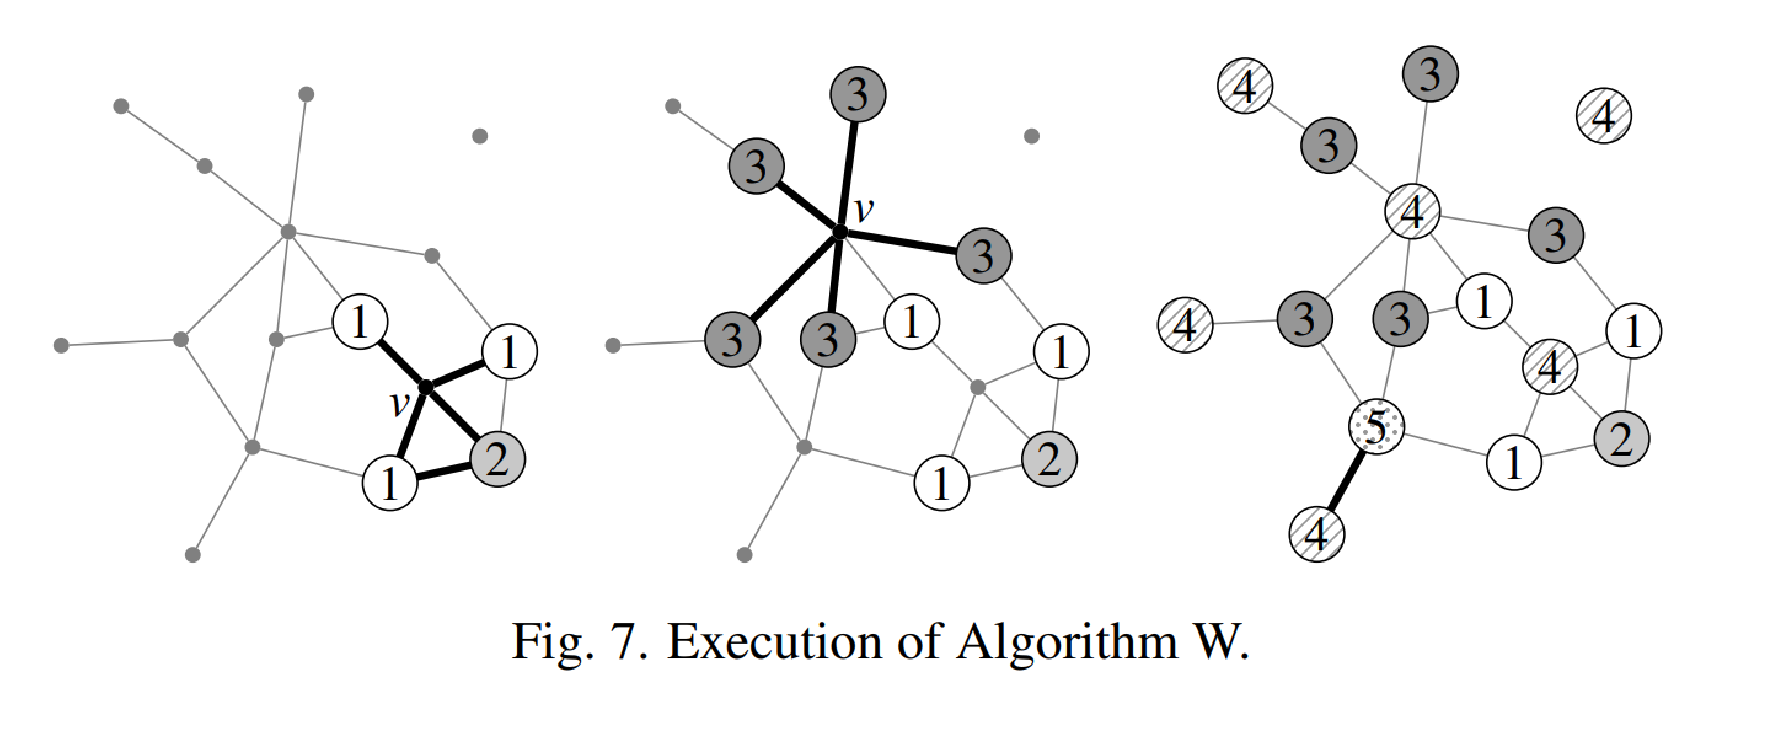
\includegraphics[width=1\linewidth]{alg_sample}
\end{center}

Это и есть алгоритм Вигдерсона \citep{Wigd}. Покажем его корректность и полиномиальность времени работы.

\paragraph{Доказательство корректности:}
Несложно заметить, что алгоритм строит правильную раскраску. Покажем, что цветов $O(\sqrt{n})$.

В каждой итерации 2 добавляется максимум 3 цвета и убирается минимум $\sqrt{n}$ вершин. Значит таких итераций не может быть больше $\sqrt{n}$ и добавится не более чем $3 \cdot \sqrt{n}$ цветов. Жадный алгоритм раскрасит оставшиеся вершины в максимум $\sqrt{n}$ цветов, то есть всего будет не более $4 \cdot \sqrt{n}$ цветов. Корректность доказана. 

\paragraph{Доказательство полиномиальности времени работы:}

\begin{enumerate}
	\item Поиск вершины с максимальной степенью~--- $O(V + E)$
	\item Покраска соседей алгоритмом $\textbf{B}$~--- $O(V + E)$
	\item $\implies$ Одна итерация цикла работает за $O(V + E)$
	\item По доказанному итераций не больше $\sqrt{|V|}$
	\item Жадный алгоритм работает $O(V + E)$
	\item $\implies$ Всего $O(sqrt{V} \cdot (V + E))$ что есть полином от количества вершин.
\end{enumerate}


Предложим полиномиальную реализацию. Подробнее - см. \citep{github}

\newpage

Фрагмент реализации на языке python.

\begin{lstlisting}[language=Python]
def wigderson_algorithm(graph):

    def apply_coloring(vertices_to_color, color_alg):
        vertices_to_color = set(vertices_to_color)
        for v in vertices_to_color:
            color_alg(graph, v, colors, vertices_to_color)
        for v in vertices_to_color:
            colors[v] += min_color
    # 1
    colors = [-1] * len(graph)
    min_color = 0
    sqrt_n = max(2, int(math.sqrt(len(graph))))
    while True:
        vertices = [v for v in range(len(graph)) if colors[v] == -1]
        if not vertices:
            break
        #2
        d, v = find_max_deg(graph, vertices, colors)
        if d < sqrt_n:
            break
        colors[v] = min_color
        min_color += 1
        curr_neighbours = neighbours(graph, v, colors)
        apply_coloring(curr_neighbours, bipartition_coloring)
        min_color = max(colors) + 1
    #3
    rest_vertices = [v for v in range(len(graph)) if colors[v] == -1]
    apply_coloring(rest_vertices, greedy_coloring)
    return colors
\end{lstlisting}


Таким образом в сумме алгоритм работает за $O(n^{2} \sqrt{n})$. Полиномиальность доказана.

\section{Заключение}
Существуют и более опримальные приближения, однако они требуют более громоздкой теории. Этот алгоритм хорош простотой реализации и довольно неплохими результатами работы (тестирование алгоритма - см. \citep{github}).

\bibliographystyle{unsrtnat}
\bibliography{references}
\end{document}
